\chapter{Write Away 6}

\begin{figure}[H]
    \centering
    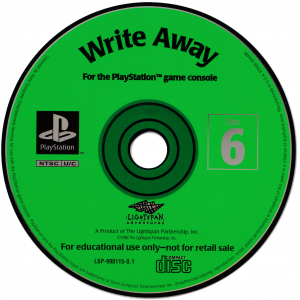
\includegraphics[width=\textwidth/2]{./Games/WriteAway/Images/WriteAway6CD.png}
    \caption{Write Away 6 CD}
\end{figure}

The sixth of the ten Write Away games published and released by The Lightspan Partnership for the PlayStation 1.

Write Away 6 features ten video programs, including an introduction video, eight story videos, and a conclusion video:

\begin{itemize}
    \item Write Away Episode Six Introduction
    \item The Vulture in the Cage by Anthony Chapparone
    \item My Friend Johnny Applesed by Matthew Barkelew and Jarrad Cole
    \item The Baby's Birthday Party by Desiree Fuller
    \item The Weird Dream by Christian Hanabergh
    \item My Sister Ate My Homework by Ben Powell
    \item A Man Named Raja by Albert Ortiz
    \item Why People Don't Go to the Cemetary at Night by Alison Heller
    \item The Invention by Jared Bowles
    \item Write Away Conclusion
\end{itemize}

\clearpage
\newpage

\section{Transcriptions}

\subsection{The Vulture in the Cage by Anthony Chapparone}

BRIAN:
Fly Away, Little Bird, be free.

SABRINA:
Brian just let a wild sparrow that he found go.
It was sick, and he nursed it back to health, but it was wild and it needed to be free.
Brian, you made the right decision.
That little Sparrow needed to be back in its home out in nature.

BRIAN:
I know, but I'll miss it.

SABRINA:
Ah, well, maybe I can cheer you up with this wonderful story about a caged animal that needed to be free.
And I bet by the end of the story, you'll know you made the right decision.
This story comes to us from Anthony Chapparone, a first grader from Midland School.
Come with us as we meet the vulture in the cage.

BRIAN (VOICE OVER):
Once upon a time, there were two vulture friends who loved to fly high up in the sky.

VICTOR:
Wawk!
Oh, Vivian, there's nothing like being free to soar high in the sky.
Woah, I love it, it's so much fun!
Woo!
And to swoop down and to eat some dead meat and then fly back up in the wild blue yonder!
I feel free!
I feel a song coming on!
[I'm free -]

VIVIAN:
Wawk!
Victor!
What's that strange robot doing over there?
He's got a cannon and a net pointed at us!
Fly Away, Victor!
Fly away!

BRIAN (VOICE OVER):
Vivian vulture got away.
But poor Victor was captured by the net and taken to a strange laboratory by a crazed robot.

ROBOT:
Now the thigh bone's connected to the leg bone, the leg bone is connected through that, ah, huh?
We need to get more parts for my bird

VICTOR:
Wawk!
Mr.
Robot, why did you put me in this cage?
I'm a wild bird, I was meant to be free, free, [for free] -

ROBOT:
Aah!
Stop that singing!
I need you to be my model.
I am going to make a robot vulture so strong and powerful it will take over the entire world!
But now we need to get more feathers.
You'll stay in this cage until I return.
Or else.

VICTOR:
No!
I wish my friend Vivian were here to help me.
What am I gonna do?

BRIAN (VOICE OVER):
Suddenly, Victor's friend Vivian appeared at the window.

VICTOR:
Vivian, it's you!
Get me out this cage!
The mad robot locked me in here!
Help me get rid of him before he takes over the world!

VIVIAN:
Wawk!
Don't worry, Victor, I'll get you out!

BRIAN (VOICE OVER):
But Vivian was too big to get through the bars.

VIVIAN:
I knew I shouldn't have eaten that last dead elk.
I know!
I'll pick the lock with my feet.

BRIAN (VOICE OVER):
So Vivian vulture picked the lock, and Victor was free.

VICTOR:
[Yay], you saved me, you saved me!

BRIAN (VOICE OVER):
But just then, the robot was coming back.
The robot entered the laboratory and became very angry.

ROBOT:
Where is my vulture gone?

VICTOR:
I'm right here, you big piece of tin!

BRIAN (VOICE OVER):
Vivian pushed the robot into the cage, and Victor locked the door.

VICTOR:
Yeah, see how you like being locked up!

ROBOT:
Waah!
Please, let me go.
I'm sorry.
If you let me go, I promise never to use wild animals for robots to take over the world again.
And I'll never use a cage to keep in those wild animals.
And I'll only make toys for children to play with.
I promise!

VIVIAN:
Yeah, let him go.

VICTOR:
All right.

ROBOT:
Oh, thank you!
Thank you!
Be free!
Be free!

BRIAN (VOICE OVER):
And so, the vultures were free to fly high up into the sky where they really belong, and they lived happily ever after.

\subsection{My Friend Johnny Applesed by Matthew Barkelew and Jarrad Cole}

PAUL:
For my next character, I'll...
I'll be happy.
That's it, happy.
Ha ha ha\dots
No, no, no.
No, no.
I'll be sad.
I'll be so sad.
Waah waah waah!
No, no, no.
No, no.
I'll be in love.
That's it.
I'll be in love.
I love you.
I love you too.
Where are you?
I'm over here.
I love you.
I love -
No, no, no.
I'll be crazy, that's it.
Weeh hee hee hee!

JOE:
Poor Paul.
He's trying to find out which mood, or feeling his next character will have.
Let's see if we can help.
Follow me, right this way.
Hi Paul, having trouble?

PAUL:
Yeah.
I can't figure out what emotion to use to make my next character come to life.

JOE:
Well Paul, you don't have to worry about your character for this next story, because he's a well-known one!

PAUL:
What do you mean?

joe:
Well, everyone has heard of Johnny Appleseed.
He's part of our American folklore.
What's really unique about this story and about writing in general is taking a character that has already developed and putting your own special twist.
That's what two authors from Alps Road School have done.
Kindergartner Jarrad Cole, and fourth grader Matthew Barkelew, have gotten this interesting character and put a new twist in their tall tale, 'My Friend Johnny Appleseed.'

NARRATOR:
This is the real story of a very unusual boy named Johnny Appleseed.
You may think my tale is tall, but once you hear it, you'll know it's true.
Johnny was a boy like any other boy, except for one thing: he loved apples.

JOHNNY:
Oh, Mom, I just love apples!
And I love the smell of apple blossoms!
And I love to pick them off the trees, and throw them up in the air, and count them all before I go to bed at night!
And, Mom, I even have dreams about apples dancing around my head!

MOM:
That's nice, Johnny boy.

NARRATOR:
One day, as he danced around the apple orchard, he came up with an idea and ran to tell his mother.

JOHNNY:
Mom, Mom!
I want to live some!
I want the whole world to loves apples the way that I do!
I'm gonna travel the countryside, and I'm gonna take seeds, and I'm gonna plant them so the trees will grow, and everybody will have as many apples as they want!

MOM:
Oh, that's nice, Johnny boy.

NARRATOR:
So off Johnny went, with apple seeds, no coat, no shoes, and only a pot to cook with.
He didn't want to carry the pot, so he wore it on his head like a hat.
A strange hat indeed.
On he went, planting seeds, until he met up with an angry farmer.

FARMER:
Hey there!
You with the pot on your head!
What are you doing on my property?

JOHNNY:
I'm planting apple seeds so you can have apples!

FARMER:
I don't like apples.
I don't like men with pots on their heads, either.
You have no right planting on my property!
For your punishment, I'm puttin' you on a train and sending you to the Wild West!

JOHNNY:
Sounds great!

NARRATOR:
And so, poor Johnny headed west.
When he got there, he met the one, the only, Pecos Bill.

PECOS BILL:
Hey there!
What do you have a pot on your head for?

JOHNNY:
It keeps the sun and the rain off my head.
Plus it's really good to make applesauce with.

PECOS BILL:
That's mighty neat!
Hey, could I have a pot from my head too?

JOHNNY:
Sure you can!
And I'll even give you some apple seeds.

PECOS BILL:
Wow\dots

JOHNNY:
My name's Johnny Appleseed.

PECOS BILL:
Pleased to meet you, Johnny.
Pecos Bill's the name.

JOHNNY:
Pecos Bill!
Hey, you're the Pecos Bill that tamed snakes and lassoed them to catch tornadoes!

PECOS BILL:
That's me!

JOHNNY:
Wow, I'd be honored if you wore my pot.

PECOS BILL:
Thanks, Johnny.
I'll pay you back real soon.

NARRATOR:
And boy, did he!
As Johnny was swimming in the Colorado River, a big, hungry fish started to chase Johnny.

JOHNNY:
Help!
Somebody help me!

NARRATOR:
Ten miles away, Pecos Bill heard screamin'.

PECOS BILL:
Sounds like my good friend Johnny Appleseed's in trouble!
I'd better go help him.

NARRATOR:
Pecos Bill pulled Johnny out just in time.

JOHNNY:
Thanks, Pecos Bill!
You saved my life!

PECOS BILL:
No problem.
Now, we're friends to the end.

JOHNNY:
To the end!
Hey, Apple?

PECOS BILL:
Oh, don't mind if I do.

NARRATOR:
And that's the tall tale of Johnny Appleseed.

\subsection{The Baby's Birthday Party by Desiree Fuller}

PAUL:
Hey, [it's neat] -
Oh hi!
Hey, we're watching a video from last year when we were at a picnic.

SCOUT:
Oh Sabrina, you won the race!

PAUL:
That's great!
You know, it's nice to look at snapshots of your family, your friends, but it's really exciting to watch an action video, because you never know what's going to happen.
What's also exciting is when an author can take a personal experience, and write it so the reader feels right in the action, just like second-grader Desiree Fuller from Conti School and her story entitled The Baby's Birthday Party.
It's me, it's me, look!

DAD:
Well, here we are at our baby's first birthday.
See, there's Junior in the chair.
That's right, say hi, Junior!
And there's Mommy, and your big brother, ha ha ha, smile.
And grandma.
Wake up, Grandma.
Grandma!
Say hi!
That's nice.
Honey, get the cake out.
Oh, will you look at that cake!
Alright, light the candle.
Oh, that's great.
    [Oh great].
Oh, love it!

Okay, blow out the candle.
Blow out the candle.
Okay, now, get a piece of cake.
The cake is in the hand.
Ha ha ha.
Ye- oh, the cake is all over them.
Oh golly!
Cake is in his ear.
Oh, the cake for mommy!
No, stop!
Oh the cake's all over grandmother's glasses.
Oh, oh, look!
Look, the cake is under the table.

Say hi, son.
Say hi.
Ha ha ha, oh this is great.
Baby's first birthday.
The end.
Wave everybody, together.
Wave!
Ha ha ha!

\subsection{The Weird Dream by Christian Hanabergh}

SABRINA:
I love to read stories about dreams that come true.
Some of them are romantic dreams about love, and some are adventure dreams about being a hero.

BRIAN:
But what if it's a strange dream that never ends?

SABRINA:
I bet if you tell me what your dream is about, I can tell you what it meant.

BRIAN:
Well, I dreamed I was on this boat going on a long voyage.
But the waves got bigger and bigger, and so I couldn't reach the shore.
What does that mean?

SABRINA:
Never take a boat, always use a surfboard.
Easy.

SCOUT:
Well, I always have the same dream of a prince that comes to my door.
He rings a doorbell, I run to answer it, but every time I open it, he's gone.
What does that mean?

SABRINA:
Never open the door without first applying lip gloss.
See?
Figuring out dreams can be easy, but sometimes they can be strange.
The great thing is that you, as an author, have complete control over how you want it to end.
That's what our next author did.
Christian Hanabergh, a third-grader from Henry Elementary, in her story The Weird Dream.

SABRINA (VOICE OVER):
Once there lived a very happy little flying fruit bat named C.H.
He and his family lived in a cave, and they just loved fruit, especially oranges.

MOM:
C.H., would you please go and fly and get us more oranges?
We're all out.

C.H.:
Yes, mother.
It's boring just hanging around here.
See you soon!

DAD:
Be sure to watch where you're going son.

C.H.:
Okay, Dad.
Bye.

SABRINA (VOICE OVER):
So C.H.
began to fly in search of oranges.
He saw an orange grove and was heading for an orange when he hit a tree and got knocked out.
The wind was so strong it picked C.H.
up and blew him far away.

C.H.:
Oh, oh no\dots
Where am I?
It's hot.
Last thing I remember I was going towards an orange tree.
Huh!
Oh no!
I'm lost!
Help!

SABRINA (VOICE OVER):
Poor little C.H.
was in a strange land with no friends or family.
He just sat in a tree and cried.
Suddenly, a funny-looking man came walking by and saw little C.H.
in the tree.

MAN:
I say, I say, what's this?
Why, why, it's a fruit bat!
Why, I'd say you've lost your way.
Come, come, no more tears.
What is your name?

C.H.:
C.H.
I was going to get some fruit from an orange tree, and then, that's the last thing I remembered.
Like some sort of weird dream, here I am.
Can you help me?

MAN:
Yes, my nocturnal friend.
I know exactly how to get you back home.

C.H.:
You do?

MAN:
Yes.
I've studied animals all my life [, yes I have].
See, you are a fruit bat.
Yes, and you have a keen sense of sight and smell.
But I'm just going to put you in a big slingshot and catapult you back where you belong.

C.H.:
Will it hurt?

MAN:
I don't know.
I've never done it before.

C.H.:
Okay, let's go.

MAN:
All right, follow me.

SABRINA (VOICE OVER):
So the interesting man put C.H.
into a giant slingshot, let it go, and off C.H.
went flying through the sky.
He flew so fast that he fell asleep.
And when he woke up\dots

MON:
Wake up, son!

DAD:
Wake up, C.H.!

You're home, son.

C.H.:
Mom, Dad, you'll never believe what happened!
I flew all the way to Africa, and then I hit my head, and some guy put me in a slingshot and flew me all the way back home!
Was it a dream?

MOM:
It was no dream, son.
It was real.
We're just glad you're back here, safe and sound.

C.H.:
Me too.

SABRINA (VOICE OVER):
And from that day on, CH always looked where he was going when he flew high up in the sky.

\subsection{My Sister Ate My Homework by Ben Powell}

SCOUT:
Oh hi!
I'm running down all the excuses in the world why homework never gets done.
And then I'll be in the Guinness Book of World Records on excuses.
And they'll have no excuse not to put me in.
I have found some great excuses, like my next-door neighbor is really an alien, and I had to take infrared pictures of her spaceship that she keeps in a big, huge Tupperware bowl, so I couldn't finish my homework.
Yeah, it's a good one.
But then there are really some lame excuses, like my dog ate it.
Huh.
Get real!
If you want to hear a really, really good excuse, one of the best ones I found came from Ben Powell, a fifth-grader from Kaiser Elementary.
He has the best excuse in the world: My Sister Ate My Homework.
Gotta write it down!

BOY:
My sister, Jenny - she's a living monster that eats homework.
Even if you tell her to stop, she doesn't listen, and just chomps away at full speed.
Jenny, stop!

JENNY:
No!

BOY:
Oh, she's homework-thirsty.
She's eating my math sheets with a side order of my social science paper.
Mom, help!

BOY (VOICE OVER):
One time, my mom locked her in her room.

MOM:
Jenny, you have to stay in your room so that you won't eat your brother's homework.
Now, go to sleep.

JENNY:
Homework.
Must have homework.

BOY (VOICE OVER):
When I woke up, there was my sister with toast and homework.

BOY:
Jenny, you're eating my homework again!

JENNY:
*burp*

BOY:
Oh, what am I gonna tell my teacher?

TEACHER:
And where is your homework, young man?

BOY:
I bumped my head, and that's why I don't have my homework done.

TEACHER:
Where did you bump your head?

BOY:
Oh, I wish just once I could turn my homework in.

BRAD:
Hey, heard your lame excuse about your homework.
Boy, you're in trouble.
He he he.

BOY:
I've got it!
I'll send Jenny to Brad's house.
She can eat his homework.
Oh, Jenny.

JENNY:
Yeah?

BOY:
Brad's got lots of homework at his house.
Decimal sheets, and math salad.

JENNY:
Hmm\dots

BOY:
He lives right over there.

JENNY:
Hmm\dots
Oh boy.
All right.

BRAD:
Hey, come back!
Hey, oh, no, don't eat it!

BOY (VOICE OVER):
This was the first time I ever turned in my homework.
But when I got home\dots

BOY:
Casey!
Oh, and you're eating my shoes!
Mom, we have a new problem!

\subsection{A Man Named Raja by Albert Ortiz}

BRIAN:
Starlight, Star bright.
First star I see tonight.
I wish I may, I wish I might, have this wish I wish tonight.
We all make wishes: on stars, when we blow out our birthday candles, when we rub magic lamps.
Some authors have wishes come true for their characters, and some authors use those wishes to teach us that we should be careful about what we wish for.
You'll see exactly what I mean in this next story by seventh-grader Albert Ortiz of Conti School, as we meet a man named Raja.

NARRATOR:
This is the story of a man named Raja.
He had no money and was not liked by anyone.

MAN 1:
Good morning, Raja.
How are you?

RAJA:
What do you care?
You have money and I have none.

MAN 1:
How rude!

NARRATOR:
Yes, Raja was rude because he envied everyone around him.
One day, Raja walked down a narrow fruitful path, where he encountered a butterfly who looked so unhappy.

BUTTERFLY:
Yes, what can I do for you?

RAJA:
You speak?

BUTTERFLY:
Well, why have you come?

RAJA:
I'm sorry, I do not know you.
I'm a stranger to this enchanted place.
All I do know is that no one loves me, or likes me.

BUTTERFLY:
He he he, oh.
That's a good one.
Tell me another.

RAJA:
I'm trying to be honest with you, but you are being rude.

BUTTERFLY:
Ooh\dots
I, sir, am a butterfly with magic powers.
And, because you have nothing, I will grant you three wishes.
But remember, seek wisely for what you wish for.

RAJA:
Three wishes?
All right.
I wish for all the money in the world.

BUTTERFLY:
Are you sure?

RAJA:
Oh, yes.

BUTTERFLY:
So be it.
Go home and speak to no one.

MAN 1:
Hello, neighbor.
How rude.

NARRATOR:
The next morning, Raja awoke filthy rich with friends.

MAN 2:
Hi!
Let's party!

NARRATOR:
But Raja soon tired of all the parties and wealth.

RAJA:
Go home.
The party is over.

MAN 2:
How rude!

NARRATOR:
He went back to the butterfly.

RAJA:
Butterfly, I am not happy with my wish.
Take it back.

BUTTERFLY:
Oh no, you cannot give it back.
But you can wish it away.

RAJA:
All right.
I wish I was poor again.

BUTTERFLY:
I'll go home and speak to no one.
Oh, you do have one more wish.
Would you like to use it?

RAJA:
No.

BUTTERFLY:
What did you say?

RAJA:
I said no.

BUTTERFLY:
Uh-huh.
You spoke when I said 'speak to no one.'
No, you will become a butterfly like me.

NARRATOR:
Raja had indeed turned into a butterfly.
But as he flew, an eagle suddenly appeared and swallowed him up.
His wishes had not brought him any happiness.
And that is the story of a man named Raja.

\subsection{Why People Don't Go to the Cemetary at Night by Alison Heller}

NARRATOR:
And now, welcome to another spine-tingling Tales From The Script.

PAUL:
Eight\dots Nine\dots Ten.
Hahaha!
Hello, my little ghoul and goulette, and welcome to another horrifically good tale of madness and mayhem!
Tonight's tale deals with a devilish dare between friends.
Will they survived Halloween?
Let's see\dots
As in this story by Alison Heller.
I dare you not to cover your eyes her a story called 'Why People Don't Go to the Cemetery at Night.'
Hahaha.

PAUL (VOICE OVER):
It was Halloween night, and four friends, Dana, David, Mike, and Kerry, were putting the finishing touches on their costumes.

DANA:
Well, how do I look?

MIKE:
Like a dead cheerleader, baby.

DANA:
Oh, good.
Ra ra ra.
Hey, you make a cool-looking clown, David.

DAVID:
Thanks.
And Kerry, you are a most excellent bride.

KERRY:
Thanks.

MIKE:
Hey, what about me?

KERRY:
Oh, well, you're a totally cool Elvis.

MIKE:
Thank you, thank you very much.

KERRY:
You're the king!
Hey?
Everybody, ready?

DANA:
Yeah, let's go.

KERRY:
Okay!

PAUL (VOICE OVER):
And so the four 14-year-olds left and went to the first house.
It looked dark, but they rang the doorbell, and an old man answered the door.

DANA, DAVID, MIKE, KERRY:
Trick or treat, smell my feet, give me something good to eat.

OLD MAN:
Hu hu, you're [a] great kid.
Here's lots of candy for ye.
Yeah, there's two for you.

KERRY:
You look creepy.
What a great costume!

OLD MAN:
It's not a costume!
Get out of here!
Grr\dots

PAUL (VOICE OVER):
And so the four fun-filled teenagers kept gathering up candy, until they came to the edge of the cemetery.

MIKE:
Hey, it's almost midnight.
Hey, Dana.
I dare you to lay down on one of the graves.
Any grave.

DANA:
Eew, do I have to?

DAVID, MIKE, KERRY:
Chicken?
*chicken noises*

DANA:
Oh, all right, I will.
But you guys have to come with me, okay?

DAVID, MIKE, KERRY:
Okay.

PAUL (VOICE OVER):
The foolish teenagers entered the graveyard and tiptoed past the graves until Dana saw one tombstone and laid down on the ground.
But suddenly, a hand came up through the ground and grabbed her.

DANA:
Aah! Aah! Aah!

PAUL (VOICE OVER):
Dana looked straight into the face of a zombie.
She jumped up, and she was surrounded.

DANA:
Aaaaah!

PAUL (VOICE OVER):
She screamed for help!

DANA:
Help!

KERRY:
Like, don't worry, I'll help you.

DANA:
Two, four, six, eight, let's get out the gate.
Come on, you guys.

PAUL (VOICE OVER):
The four teenagers ran out of the cemetery and then looked back.

MIKE:
Look!
The zombie can't get past the cemetary walls.
He's going back to his grave!
We're safe.
Come on, let's go home.

DANA:
I don't think anyone will ever believe us.

KERRY:
Like, we can never tell anyone.

MIKE:
I don't think we'll ever recover.

DAVID:
Do you think it was real?

PAUL (VOICE OVER):
They would often think and wonder if it was real, but Carrie never got her high heel back.
Dana's pom-pom was lost forever, and David and Mike kept having the same bad dream.
And that, my friends, is why people are afraid to go to the cemetery at night.

PAUL:
Now wasn't that a hair-raising tale of terror?
I know I'll think twice before I dare anyone to do something as fun as romp through a cemetery uninvited.
Hahaha.
Well, goodbye for now, and I dare you not to keep in touch.
Hahaha.

\subsection{The Invention by Jared Bowles}

JOE:
All right, my pet hamster Melvin is ready to race in this new race car invented just for hamsters.

PAUL:
Yeah, well my guinea pig go-kart is spectacular and ready for action.

JOE:
Oh, hi!
We have no time to chat.
We have a race to start.

PAUL:
Oh, we have a minute.
As inventors, we like to invent things that are useful for mankind - inventions that help, not hurt.

JOE:
And as writers, you are inventors.
By using your imagination, you can create stories that help us learn more about ourselves and others.

PAUL:
And we'd like to honor you inventive minds out there with a story about a man who invented the ultimate machine.

JOE:
Comes to us from fourth grader Jared Bowles from Fryberger Elementary.
Now, we introduce you to the invention.

PAUL, JOE:
Ready? Set? Go!

SABRINA (VOICE OVER):
Once upon a time, there was an inventor named John, who was a terrific inventor.
He was getting interviewed on a show to explain his new invention.

TELEVISION PRESENTER:
Tell us, Professor John - may I call you that?

JOHN:
Oh, absolutely.
Anything you like.

TELEVISION PRESENTER:
Tell us a little bit about your inventions and how they work.

JOHN:
I'd love to!
Right, this is a light bulb.
I invented this to bring light into the world.
Hahaha!
You just put it in the socket and voilà, light!

TELEVISION PRESENTER:
And what's that right there.

JOHN:
Oh, oh, this?
This is an ordinary pencil.
Yeah, I was in a writing mood when I invented this.
Hahaha!
Get it?

TELEVISION PRESENTER:
Yes, I do.
Now tell us a little bit about your new invention.

JOHN:
Oh I'd love to.
This is called Live Again!
It'll take anything that's sick and make it healthy.
For instance, take this very sick-looking flower.
Alright, I put it in here, and I pull the lever.
And look!
Oh, it's well again!

TELEVISION PRESENTER:
Oh, that's amazing!

JOHN:
I know!

TELEVISION PRESENTER:
Oh, good luck, good luck.
And please stay tuned with us tomorrow when we have a man on the show who says he knows the reason why hot dogs explode in the microwave!
So, see you tomorrow, bye!

SABRINA (VOICE OVER):
And so John went home excited.
There he found his son Junior working hard.

JOHN:
Will you stop working!
Hey, did you see me on TV?

JUNIOR:
Yes dad.

JOHN:
I looked pretty good, didn't I?

JUNIOR:
Yes, dad.

JOHN:
I want to celebrate.
Let's go up to the mountains in the snow and have some fun.

JUNIOR:
Okay, dad.

JOHN:
Come on.
Why Junior, with this invention, we can heal everybody who's sick and make everybody happy.

JUNIOR:
And I helped!

JOHN:
Yes, you did, Junior.
Why, you're the best assistant and the best son an inventor could want to have.
Not to mention the best guinea pig.
All my inventions are a success because -

JUNIOR:
I helped!

JOHN:
That's right, Junior.
Oh, here we are.
Let's go out in the snow and have some fun.

SABRINA (VOICE OVER):
But just as the professor and his son were about to build a snowman, they heard a noise.

YETI:
Raaar!

JOHN:
[Oh], what's that sound, Junior?

JUNIOR:
I'll go see.

JOHN:
Don't talk to strangers!

SABRINA (VOICE OVER):
It was a bear.
A bear that was a little too friendly.

JOHN:
Oh, shoo!
Get away, bear, get out of here!
Oh, son, son, are you all right?
I'll take ya back to the car and take ya home.
Oh, this is the perfect time to see if my invention really works.
Come on, get on my back.
Let's go.
Son, you have to sit up if you want your dad to be able to drive right.

JUNIOR:
And I helped.

JOHN:
Yes son you did.
Oh, we're here.

SABRINA (VOICE OVER):
John had to hurry and put Junior in the machine.
He turned on the lever, and suddenly Junior jumped out as good as new.

JOHN:
Oh, it works!
It really works!
Now, people can use this machine to make everybody well.

JUNIOR:
And I helped!

JOHN:
Yes, you did, Junior.

SABRINA (VOICE OVER):
And they lived happily ever after.

\subsection{Write Away Conclusion}

SCOUT:
Well, it's that time again.
Time to say goodbye until we see you next month.

JOE:
Let's see\dots
We've seen action with the vulture, and the whole movie of a birthday party.

SABRINA:
Zombies and butterflies, and kids who eat homework.

BRIAN:
Johnny Appleseed and Pecos Bill, and strange bats in strange places.

PAUL:
And you've seen all this because you've used your imagination to bring it all to life.

JOE:
So who knows what you could come up with next.
The possibilities are endless.

SABRINA:
Keep writing about anyone and anything that comes to your mind, and send it to us.

BRIAN:
Come on, do it now!

SCOUT:
And we'll keep looking for those great stories.
Until then\dots

EVERYONE:
right away!

\section{Credits}

Executive Producers: Gregg Baker, Deborah Brucher Wren, Michael Wren;
Directors: Gregg Baker, Robin LeValley;
Technical Director: Joseph S. Abreu;
Cast: Paul David, Scout Jackson, Joe Lopez, Jr., Sabrina Lu, Brian Kwan;
Writers: Deborah Brucher Wren, Robin LeValley;
Music: Rick Illes, Michael Wren;
Lighting Director: Steve Raines;
Cameras: Bill Bork, Mike Conners, Richard Crow;
Audio: Rad Corn;
Childrens Art: Blythe Baker;
Production Assistant: Sam Kephart;
Editor: Joseph S. Abreu;
Engineer: Michael Curran;
Production Coordinator: Judy Block;
Graphic Artist: Alan Scott;
Theme Song: Michael Wren;

\clearpage
\newpage

\section{Screenshots}

\begin{figure}[H]
    \centering
    \begin{subfigure}{0.45\textwidth}
        \centering
        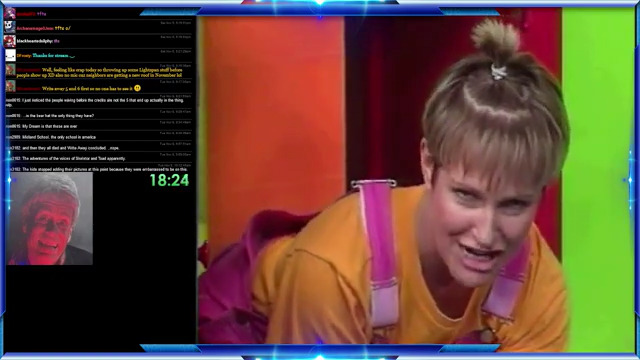
\includegraphics[width=\linewidth]{Games/WriteAway/Images/WriteAway6Screenshot1.jpg}
        \caption{Write Away 6 - Screenshot 1}
    \end{subfigure}
    \begin{subfigure}{0.45\textwidth}
        \centering
        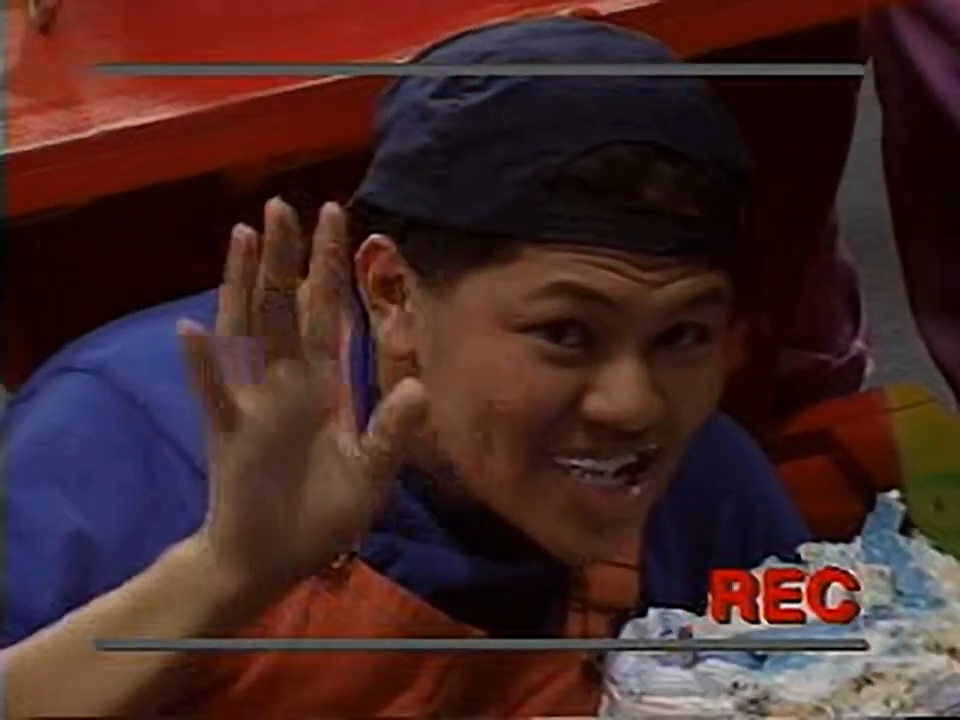
\includegraphics[width=\linewidth]{Games/WriteAway/Images/WriteAway6Screenshot2.png}
        \caption{Write Away 6 - Screenshot 2}
    \end{subfigure}

    \begin{subfigure}{0.45\textwidth}
        \centering
        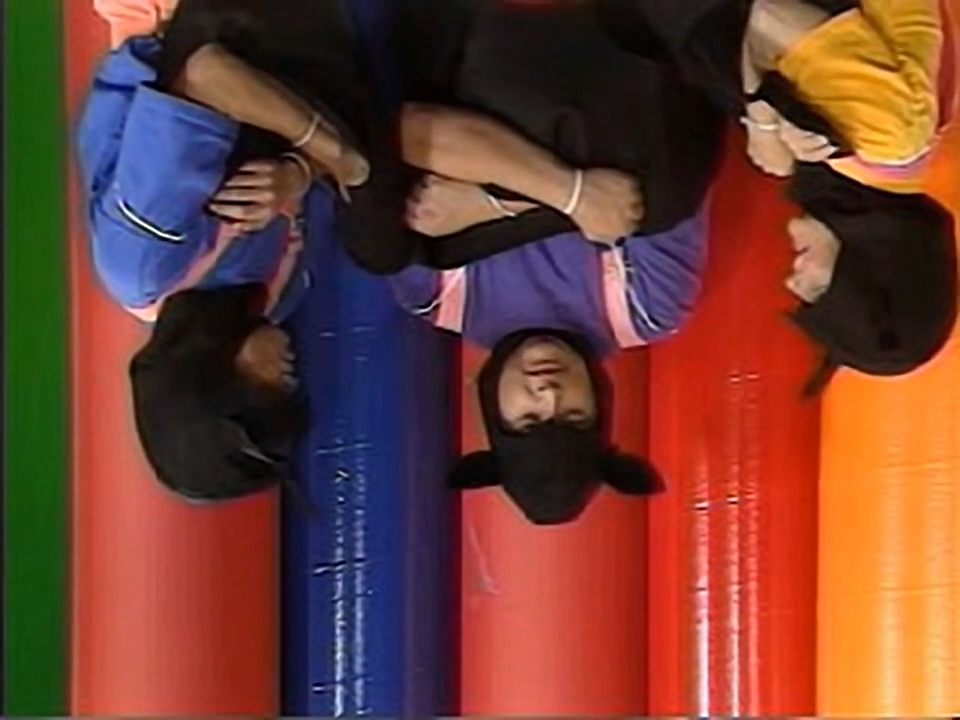
\includegraphics[width=\linewidth]{Games/WriteAway/Images/WriteAway6Screenshot3.png}
        \caption{Write Away 6 - Screenshot 3}
    \end{subfigure}
    \begin{subfigure}{0.45\textwidth}
        \centering
        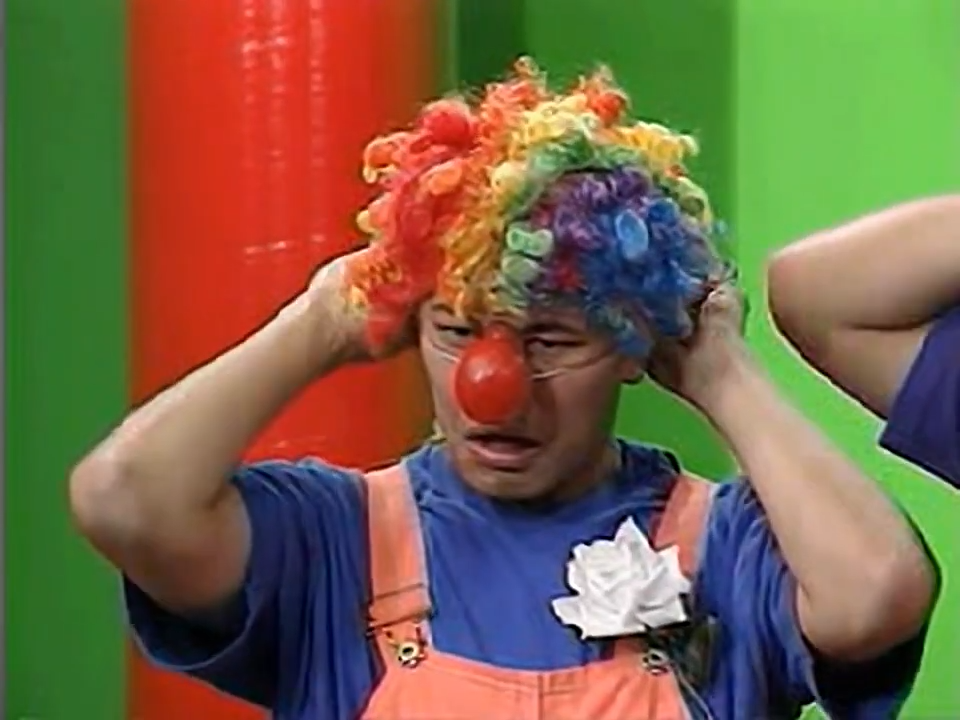
\includegraphics[width=\linewidth]{Games/WriteAway/Images/WriteAway6Screenshot4.png}
        \caption{Write Away 6 - Screenshot 4}
    \end{subfigure}
    \caption{Screenshots from Write Away 6}
\end{figure}
